%#!platex --src-specials main.tex

\chapter{仮想触覚提示手法}

本章では仮想触覚を提示するための手法について説明する.
\section{概要}
これまで振動によるテクスチャ再現の研究は数多く行われており,その振動
刺激は再現性の高いものとなっている.しかし,そのほとんどが再現時
は1方向の振動に限定されている.本研究ではこの振動方向に注目し,
X軸とY軸の二次元振動情報の記録手法と,記録した振動を
可能な限り正確に再現する振動提示手法について述べる.


\section{記録}

\subsection{記録したテクスチャ}
今回の実験では,天然芝に近いやわらかい人工芝のテクスチャ,
天然芝と異なり突起が多くチクチクした人工芝のテクスチャ,
硬めの絨毯のテクスチャ,やわらかめの絨毯のテクスチャ,
PLA(Polylactic Acid)製のタイル模様の自作テクスチャ,
目が粗くざらざらした40番の紙やすりのテクスチャ,
それぞれ材質の異なるランチョンマット3種のテクスチャ,
ツルツルした板に無数のパンチ穴が開いているテクスチャ
の10個のテクスチャの振動情報を記録した.
タイルテクスチャについて自作したテクスチャを使用している理由については後述する.
記録したテクスチャを図\ref{4-4}に示す.なお本実験では上段の左から人工芝1,人工芝2,
カーペット1,カーペット2,タイルとし,下段の左から紙やすり,ランチョンマット1,
ランチョンマット2,ランチョンマット3,プラスチックパンチとする.

\begin{figure}[h]
\begin{center}
  \includegraphics[width=10cm]{texture.eps}
  \caption{振動情報を記録したテクスチャ}
  \label{4-4}
\end{center}
\end{figure}

\subsection{記録手法}
まず,テクスチャの振動情報の記録手法について説明する.
指に3軸加速度センサ(ADXL-335)をテープで固定し,
その指で実際のテクスチャを触察した時に発生する加速度情報を記録する.
記録者は一人(20代,男性)である.
テクスチャをなぞる速度が約\ 5\ cm/s一定になるようメトロノーム
を用いて調整しながら振動記録を行った.また,各テクスチャに対して
左から右と上から下の2方向の振動を記録した.なお,人工芝1に関しては他のテクスチャに比べ指を動かす
方向によって大きく振動が異なるテクスチャであるため,右から左と下から上の方向も含めた4方向の振動
を記録し実験に使用した.

振動情報の記録の様子を図\ref{4-1}に示す.

\begin{figure}[h]
  \begin{center}
  \includegraphics[width=10cm]{collect1.eps}
  \caption{振動情報の記録}
  \label{4-1}
\end{center}
\end{figure}



実際に記録した振動情報の一部を図\ref{4-5},図\ref{4-6}に示す.
図\ref{4-5}が人工芝1を記録したもの,図\ref{4-6}が人工芝2を
記録したものである.
\begin{figure}[h]
\begin{center}
  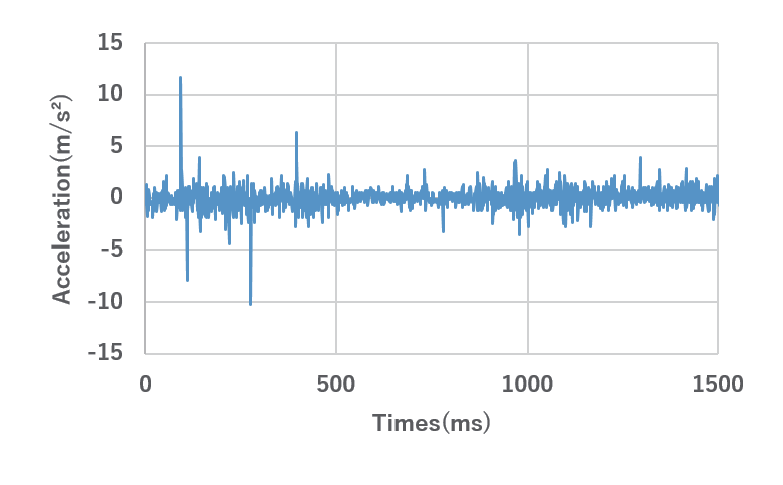
\includegraphics[width=12cm]{grass1.eps}
  \caption{記録した人工芝1の振動情報}
  \label{4-5}
\end{center}
\end{figure}

\begin{figure}[h]
\begin{center}
  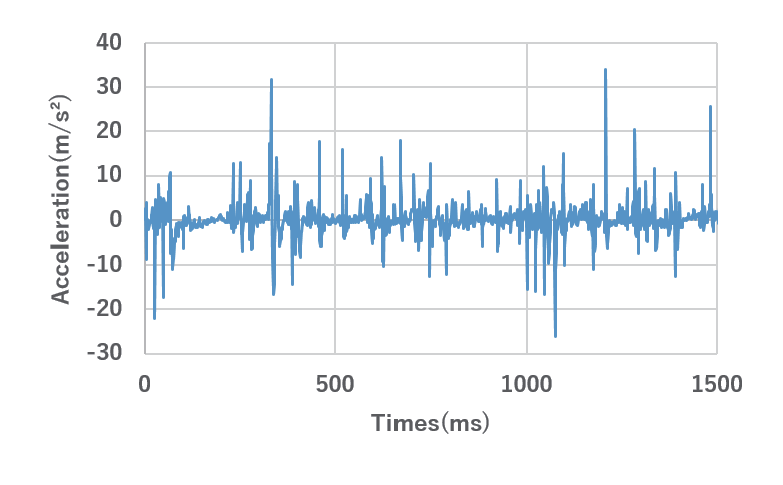
\includegraphics[width=12cm]{grass2.eps}
  \caption{記録した人工芝2の振動情報}
  \label{4-6}
\end{center}
\end{figure}
\newpage

\subsection{シリアル通信}
Sagaら\cite{saga2013simultaneous}は加速度情報を音声入力
で記録していたため1次元のデータとして記録されていた.
本研究では,3次元のデータを正確に取得するため,加速度センサを接続した
Arduinoからシリアル通信を利用して加速度情報をPCへ送信し,
PC側ではProcessingにより送信された振動情報を記録した.
図\ref{4-2}にシリアル通信の流れを示す.
振動は通信速度の関係で約\ 1\ kHzでサンプリングされる.

\begin{figure}[h]
\begin{center}
  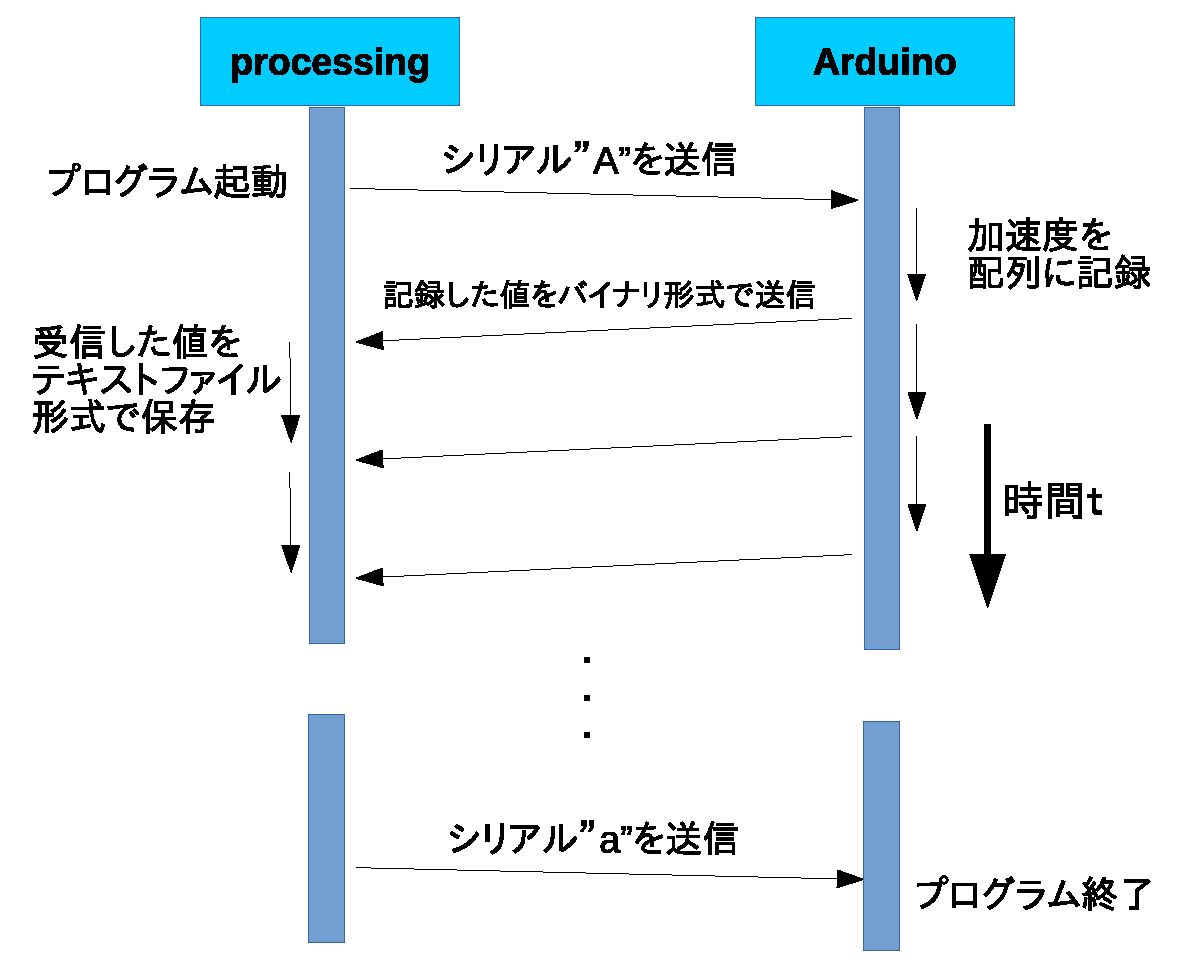
\includegraphics[width=10cm]{bainari.eps}
  \caption{シリアル通信}
  \label{4-2}
\end{center}
\end{figure}
また,データの送信の際に通常のテキスト形式で送信するとデータのサイズが大きく
なり,通信速度が遅くなってしまう.そこで今回はデータをバイナリ形式で
送信することで通信速度を向上させている.図\ref{4-4}に
テキスト形式のデータををバイナリ形式のデータに変更した場合の
具体的なデータサイズの変化を示す.
\begin{figure}[h]
\begin{center}
  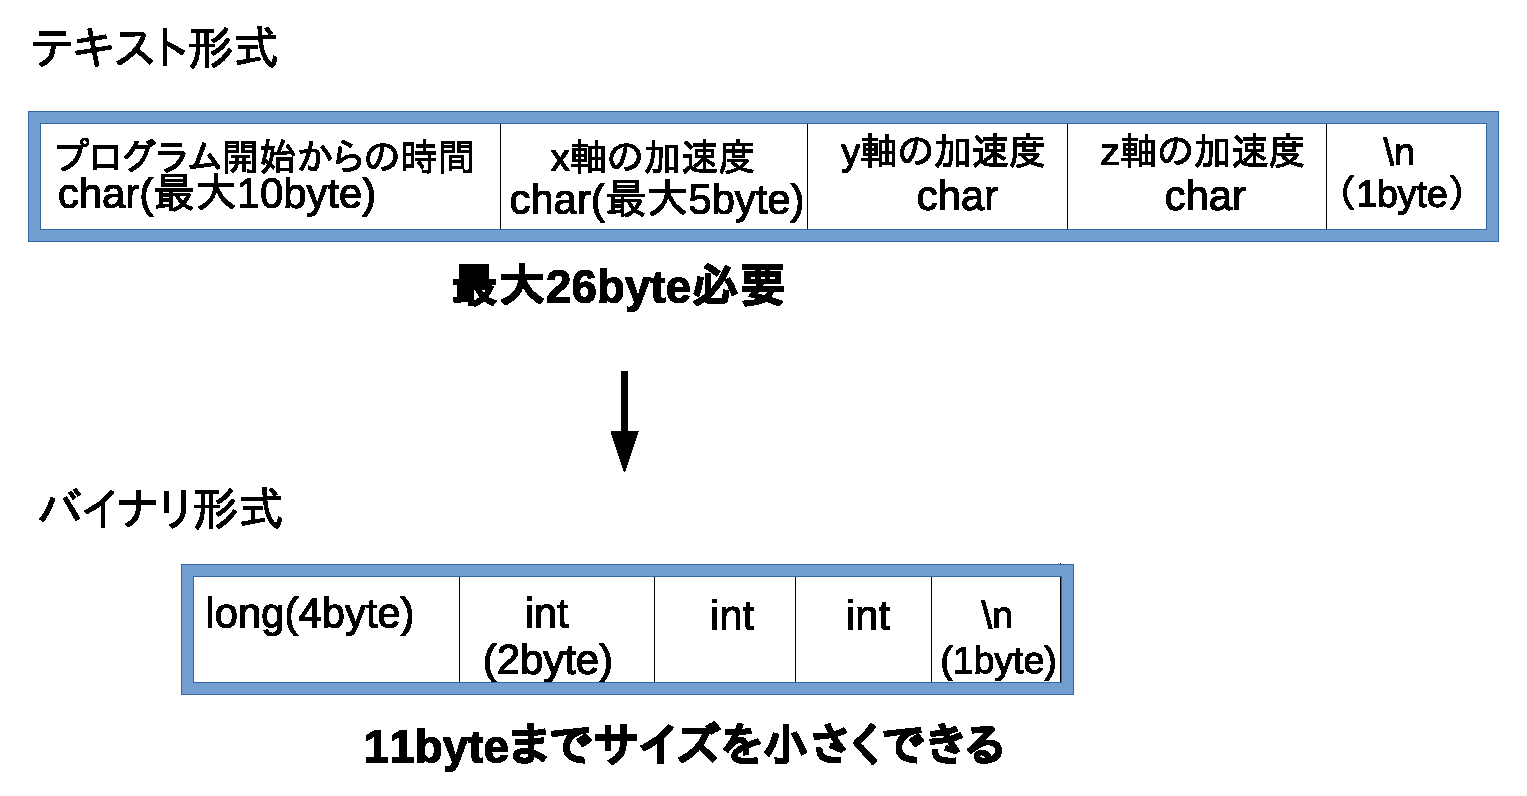
\includegraphics[width=11cm]{binary.eps}
  \caption{テキスト形式をバイナリ形式に変更したときのデータ量の変化}
  \label{4-4}
\end{center}
\end{figure}

\subsection{指の移動方向}
我々は,記録された振動方向を正確に再現する提示手法を提案し,
これを検証する.先行研究\cite{saga2013simultaneous}
により明らかにされているように,
移動方向と振動方向の関係には,提示する刺激によっては大きな再現性
の損失をもたらすことが知られている.そこで記録された振動方向を正確に提示し,
より忠実な振動を再現するためには,指を動かす方向によって,
それぞれの移動方向にとって適切な振動を再現する必要がある.
我々は,以前に上下左右の4方向に指を動かした場合の振動情報を別々に記録し,
再生時の指の方向に即した振動を選択して提示する手法を提案した.
しかし,この手法では4方向の振動が指の移動方向により逐次切り替わって提示されるため
,ランダムな空間周波数をもつ振動が生成されやすく,いくつかのテクスチャに対して再現性が
低くなってしまうという問題点があった.
そのため,本研究では振動情報の記録時に,X軸とY軸方向の2方向に指を動かした場合の
振動を記録した.これにより,指の移動軸による振動の変化を再現しつつ,提示振動の
切り替えを最小限にすることでランダムな空間周波数をもつ振動の生成を軽減することが可能となる.

再現手法については次節にて詳説する.


\section{提示手法}
振動の再現はあらかじめ2方向の触察時に記録した対象と指との間で発生する振動
と,スクリーン方向に剪断力を提示可能な,剪断力提示装置を用いて行う.
2.4.2節で紹介した補償手法では,
記録時の指の移動速度と再生時の移動速度の比を用いて
信号の再サンプリングを行っていた.本研究では,指を動かす方向
によって,それぞれの移動方向にとって適切な振動を再現する提示手法を提案し,
これを用いて実験を行う.以下ではこの提示手法について記述する.\par
あらかじめ記録する振動情報として指をテクスチャ平面上で左から右と上から下の2方向
に動かした場合の振動情報を記録した.提示時には,これら2方向の振動情報を
利用することで振動パターンを生成し,これを提示する.提示手法
としては様々考えられるが,我々は,振動がどのようにして発生するかに着目し
,発生要因に応じた振動を生成する手法を提案する.すなわち,振動とは,
触察によって初めて生起する現象であり,触察の移動方向に応じて異なる
振動に対して移動方向でパターン分けを行う.今回の実験では以前にSagaら\cite{saga2013simultaneous}
が提案した手法を参考にした補償手法を用いる.
以下にその補償手法を記す.\par
まず,記録および再生する情報を定義する.ここで,記録する情報と
加速度および指位置の記録は対象と指とのX,Y軸の2方向への相対運動
を独立に取得する(添字の$\mathcal{D} = \{X,Y
\}$は移動方向,$r, p$は記録時と再生時を表す).

\begin{eqnarray}
\mathbf{a}_{r}^\mathcal{D}(t_{r})=\left(\begin{matrix}a_{rx}^\mathcal{D} \\ a_{ry}^\mathcal{D}\end{matrix} \right)\\
\end{eqnarray}
この$t_{r}$は記録時の時間.
また,再生時の指位置の記録$\mathbf{X}_{p}$を取得し,この値をもとに指の移動速度を導く.
\begin{eqnarray}
\mathbf{X}_{p}(t_{p})=\left(\begin{matrix}x_{p}\\y_{p}\end{matrix}\right)\\
\end{eqnarray}
このとき,再生時の指の移動速度$\mathbf{\dot{x}_{p}}$はタッチスクリーンのフレーム間時間差$\Delta T$,
単位時間$\Delta T$での移動距離$\Delta\mathbf{X}_{p}(t_{p})$を用いて,

\begin{eqnarray}
\mathbf{\dot{x}_{p}}=\frac{\Delta\mathbf{X}_{p}(t_{p})}{\Delta T}=\left(\begin{matrix}\frac{\Delta x_{p}}{\Delta T}\\\frac{\Delta y_{p}}{\Delta T}\end{matrix}\right)
\end{eqnarray}
のように表せる.
また,再生時には記録時の適切なタイミングの振動を提示するため,記録時の移動速度$\mathbf{\dot{x}_{r}}$と再生時の指の移動速度$\mathbf{\dot{x}_{p}}$
の比を用いて提示すべき振動は,
\begin{eqnarray}
\mathbf{a}_{p}^\mathcal{D}(t_{p_{n+1}}) &=& \mathbf{a_r}^\mathcal{D}(t_{p_{n}} + \frac{|\mathbf{\dot{x}_p}(t_{p_{n}})|}{|\mathbf{\dot{x}_r}(t_{p_{n}})|} \Delta {T})
\end{eqnarray}
となる.なお,本実験においては$\mathbf{\dot{x}_{r}}$ = \ 5\ cm/sで一定とした.なお,
図 \ref{4-3}に示すように,移動方向に応じて,
$\mathbf{a}_{p}^\mathcal{D}(t_{p_{n+1}})$の$\mathcal{D} = \{ X,Y \} $の信号
から用いる加速度情報を切り替え,提示する.
斜め方向への移動の際は,移動距離の$x, y$成分の大きさに応じて2つの振動の線形和をとって提示する.
$\alpha$をX軸方向の移動成分,$\beta$をY軸方向の移動成分とすると,
以下の式を用いて提示する加速度$\mathbf{a}_p(t_{p_{n+1}})$が求められる.
\begin{eqnarray}
\mathbf{a}_p(t_{p_{n+1}})=\displaystyle\left|\frac{\alpha}
{\sqrt{\alpha^2+\beta^2}}\right|\mathbf{a}_{r}^{X}
(t_{p_{n+1}})+\left|\frac{\beta}{\sqrt{\alpha^2+\beta^2}}
\right|\mathbf{a}_{r}^{Y}(t_{p_{n+1}})
\end{eqnarray}

\begin{figure}[h]
\begin{center}
  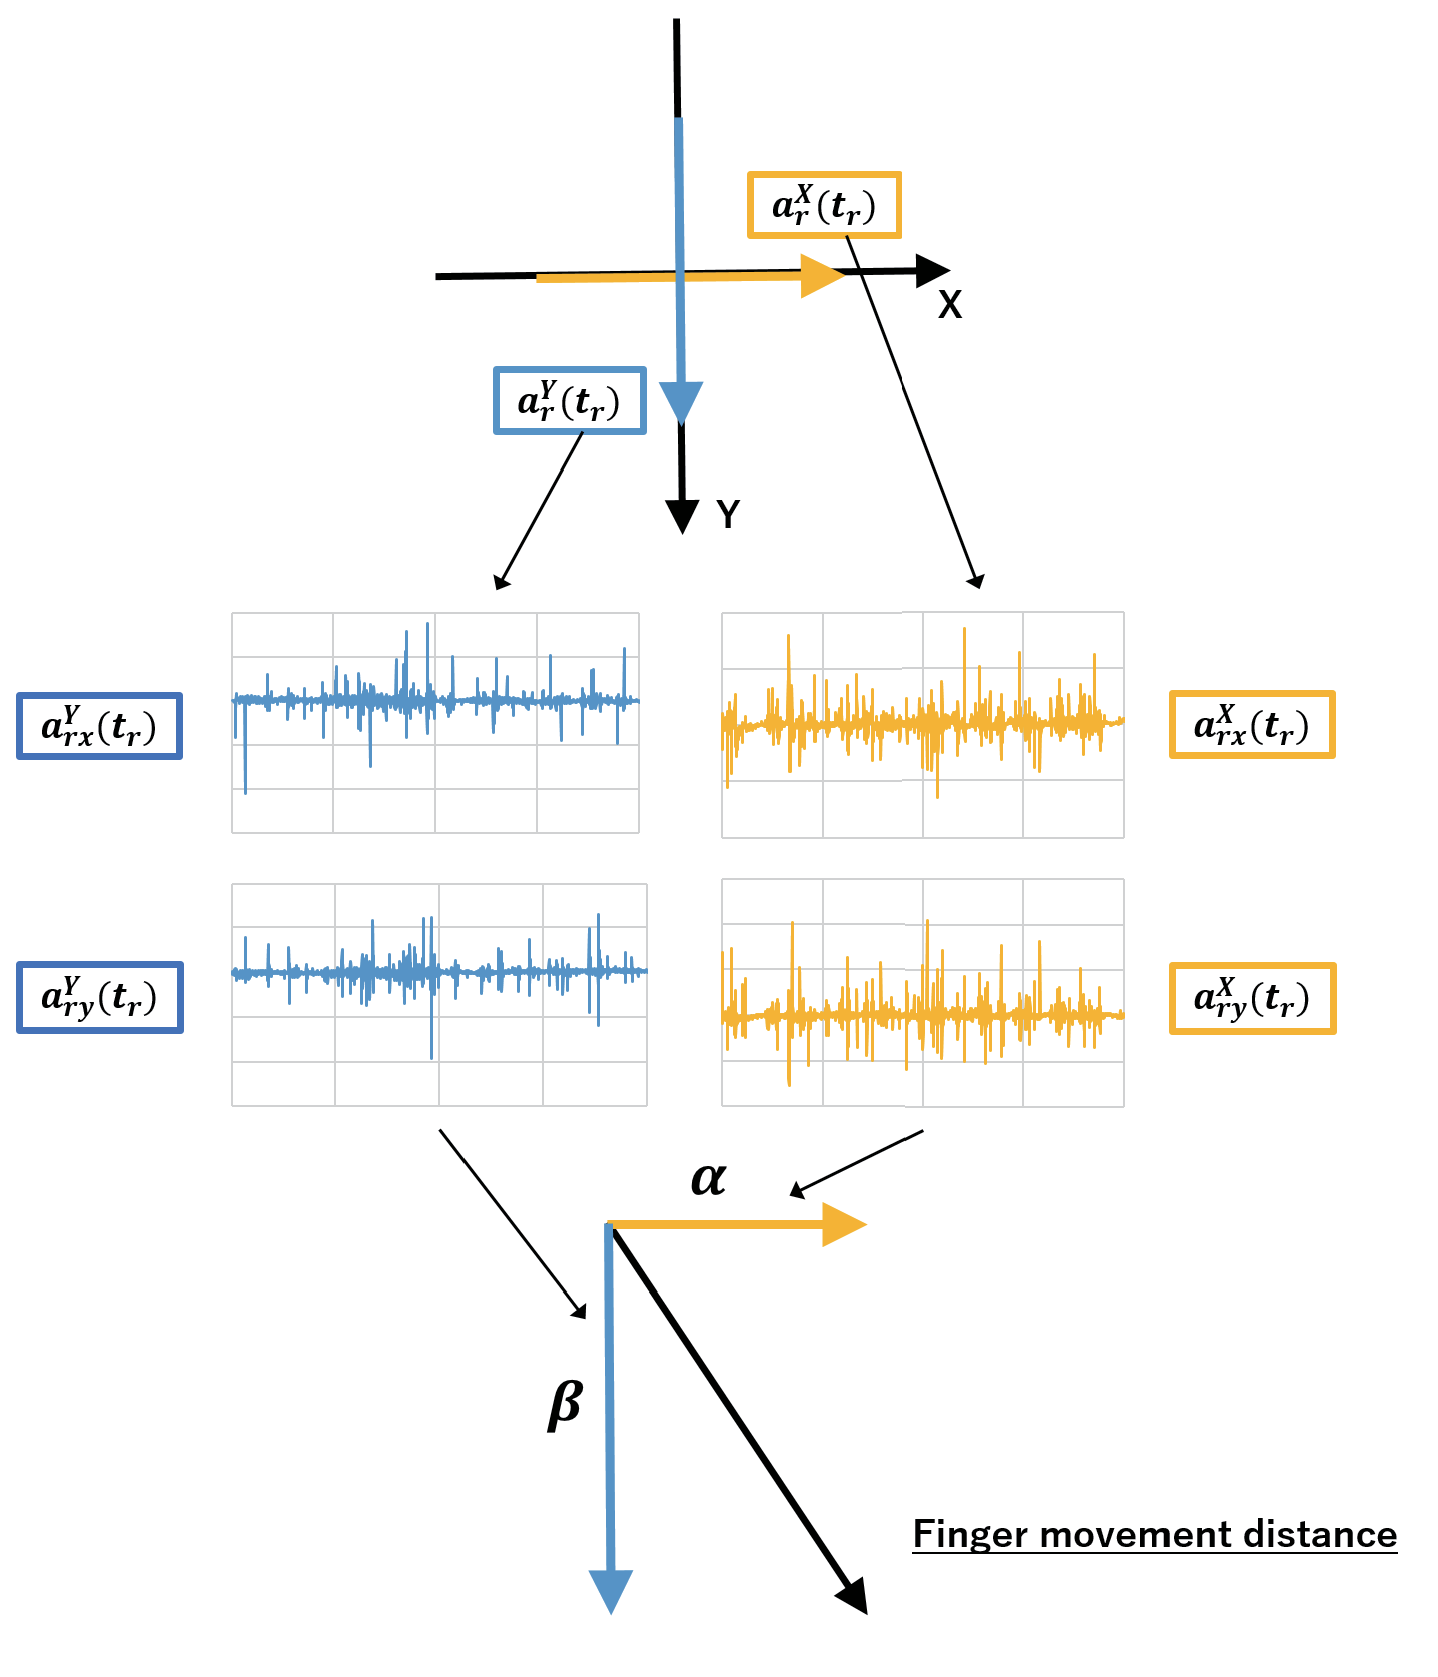
\includegraphics[width=12cm]{move.eps}
  \caption{指の移動方向に応じた振動の提示手法}
  \label{4-3}
\end{center}
\end{figure}

\section{画像特徴量の重畳を用いた振動提示手法}
前節にて提案した振動提示手法は,2方向の振動を記録しておき,指の移動成分に応じて2つの振動を適宜
組み合わせて振動を提示する.
記録する方向を2方向に限定することで提示振動の切り替えを最小限にし,ランダム性の高い空間周波数
をもつ振動の生成を低減したが,振動の切り替えや2つの振動の線形和をとる段階で提示振動の
空間周波数がランダム性をもってしまうことは避けられない.
これは一定の空間周波数をもつテクスチャを再現する際に障害になってしまう.そこで,我々は記録振動をそのまま
提示するのではなく,画像情報を用いて提示振動がランダムな空間周波数をもたないようにすることでこの問題を解決する.
我々は振動提示に利用可能な情報としてテクスチャの画像情報に着目した.本稿ではそのなかでも特に
画像特徴量を用いた振動提示手法を提案する.
\subsection{画像特徴量の取得}
画像特徴量はOpenCV等のライブラリを用いて画像処理
を行うことで取得することができる.
画像から抽出される画像特徴量にはsizeやangleといったパラメータが格納されており,それらの情報はテクスチャの特徴を
表すデータである.そこで本手法ではこれら特徴量に含まれる情報を抜き出して振動提示に利用できる一次元の形に
加工し,振動情報に重畳することで特徴的な部分をより強調した振動提示を可能にする.画像特徴慮取得の手順を
以下に示す.


\begin{enumerate}
 \item AKAZEを用いてテクスチャ画像から特徴量を取得
 \item 特徴量周辺の重要領域の直径を表すsizeの情報を抜き出す
 \item x軸,y軸方向に平均をとることで1次元の情報に加工する
 \item 最小値0,最大値1で正規化することで振動情報に重畳可能な形にする
\end{enumerate}

本章では空間周波数が一定のテクスチャとしてpolylactic acid(PLA) 製のタイル模様の自作テクスチャ画像から
画像特徴量を取得する.自作テクスチャを使用している理由として,以前の研究で使用していた樹脂製のタイル
テクスチャがスティックスリップ現象を発生しやすく,再現が困難な素材であったことと,表面に光沢がありランバート面からほど遠い
テクスチャであり,画像処理に適さない素材であったため,今回は試験的に3Dプリンタで自作したタイル模様テクスチャを使用している.

実際に使用した自作テクスチャを図\ref{tile}に,そのテクスチャに対して特徴量抽出をおこなった結果を図\ref{akaze}に示す.

\begin{figure}[ht]
\begin{center}
  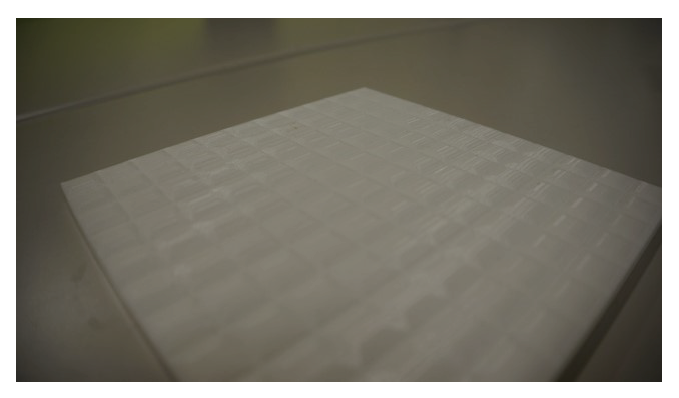
\includegraphics[width=12cm]{tile.eps}
  \caption{PLA(polylactic acid) 製のタイル模様の自作テクスチャ}
  \label{tile}
\end{center}
\end{figure}

\begin{figure}[ht]
\begin{center}
  \includegraphics[width=12cm]{AKAZE.eps}
  \caption{AKAZEを用いて抽出した画像特徴量}
  \label{akaze}
\end{center}
\end{figure}

また,抽出したsize情報を一次元の情報に加工して正規化したものを図\ref{kpx}に示す.

\begin{figure}[ht]
\begin{center}
  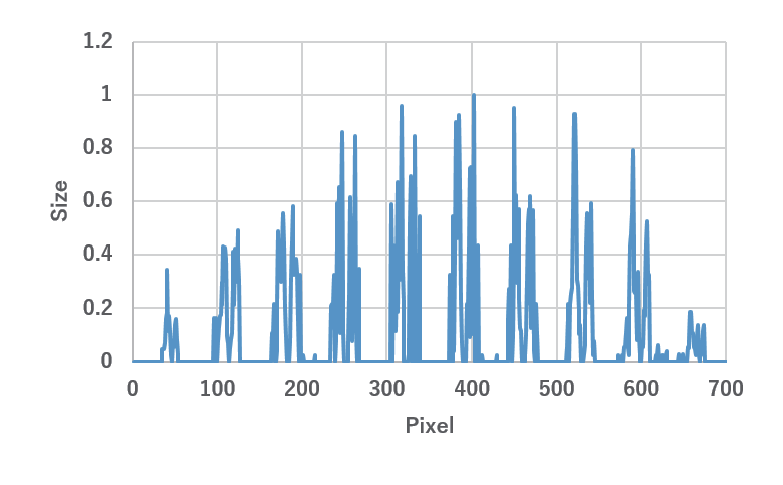
\includegraphics[width=12cm]{kpx.eps}
  \caption{自作タイルテクスチャから抽出したパラメータ $e_x0(x)$}
  \label{kpx}
\end{center}
\end{figure}

図\ref{kpx}を見るとタイルの溝の部分に対応するように特徴点が集まっていることが分かる.
しかし,この方法では多く特徴点が集まっている部分とそうでない部分とで特徴点でもsizeの大きさに
違いが出ている.これをそのまま振動情報に重畳すると特徴点間で振動の強弱が出てしまう.
そこで画像特徴量を正規化する前に対数関数logをとることでこの特徴点間の出力の強弱を
軽減する.また画像特徴量を最小0,最大1で正規化している関係で,画像特徴量
を重畳する際に記録した振動情報が損失してしまうという問題も対数関数を用いることで軽減される.
対数関数を用いて求めた画像特徴量を図\ref{kpxlog}に示す.
\begin{figure}[ht]
\begin{center}
  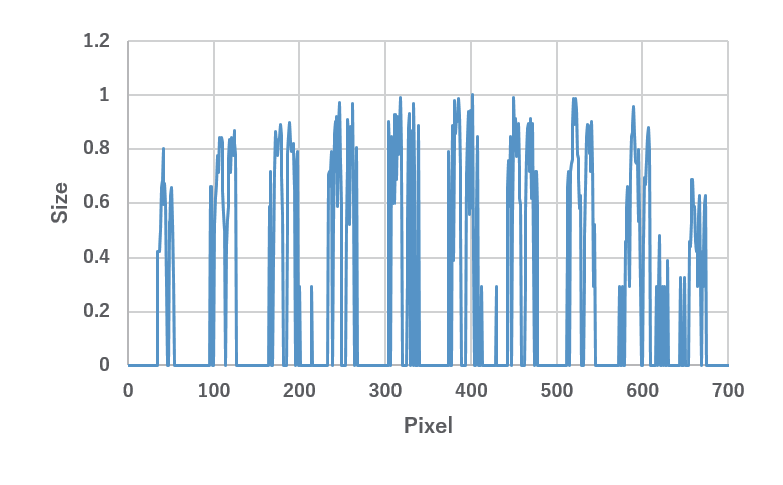
\includegraphics[width=12cm]{kpxlog.eps}
  \caption{ パラメータ$e_x0(x)$ に対数をとったパラメータ $e_x1(x)$}
  \label{kpx}
\end{center}
\end{figure}

\subsection{画像特徴量を重畳した振動提示}

提示振動$a(x,y)$は以下の式で求められる.この時$x,y$はそれぞれの座標,$a_x,a_y$はx軸,y軸の提示振動,
$F_{akaze}.size (x, y)$を画像特徴量としたとき,
$e_{x0},e_{y0}$は$F_{akaze}.size (x, y)$をそれぞれY軸とX軸方向に平均をとったパラメータであり,$e_{x1},e_{y1}$は
$e_{x0},e_{y0}$にさらに対数をとったパラメータである.なお,$a_x,a_y$は3.3節において求めた加速度である.
\begin{equation}
  e_x0(x)=\frac{1}{y} \sum_y F_{akaze}.size (x, y)
 e_y0(x)=\frac{1}{x} \sum_x F_{akaze}.size (x, y)
 e_x1(x) = log e_x0(x)
 e_y1(x) = log e_y0(x)
 a(x, y) = axex*(x) + ayey*(y)
\end{equation}

図\ref{acc1}に画像特徴量を重畳する前の自作タイルテクスチャの振動情報を示す.
図\ref{acc2}に画像特徴量を重畳した後の振動情報を,
図\ref{acc3}に対数関数を用いて正規化した画像特徴量($e_{x0}, e_{y0}$) を重畳した後の振動情報を示す.

\begin{figure}[ht]
\begin{center}
  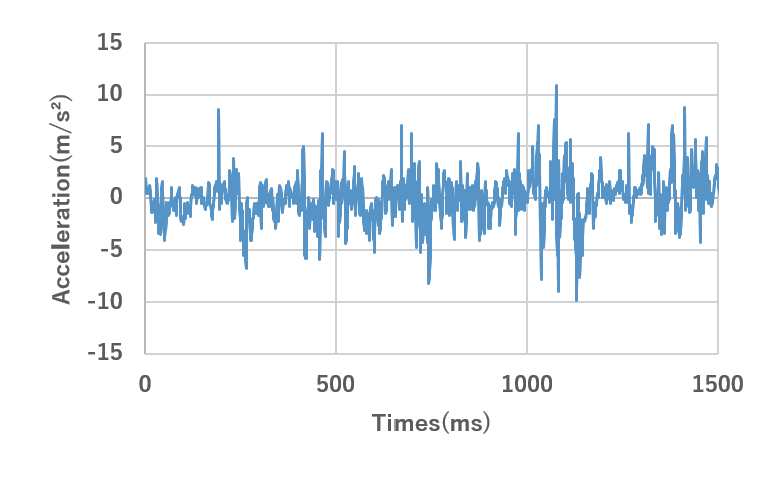
\includegraphics[width=12cm]{acc1.eps}
  \caption{パラメータ$e_x0(x)$を重畳する前の自作タイルテクスチャの振動情報}
  \label{acc1}
\end{center}
\end{figure}


\begin{figure}[ht]
\begin{center}
  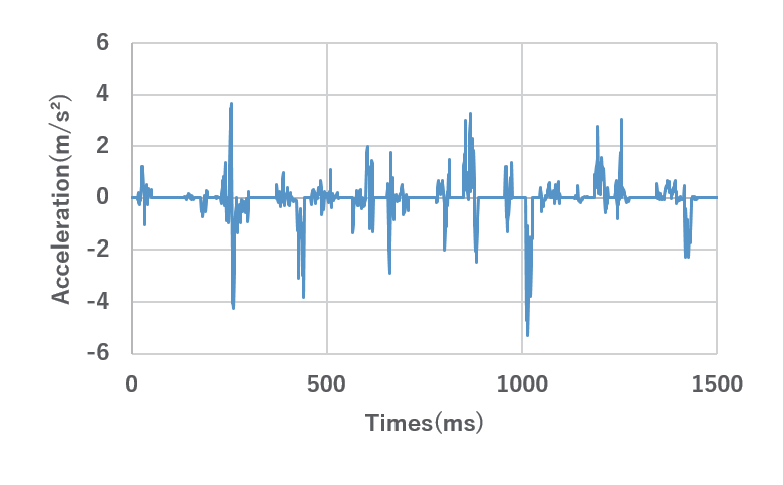
\includegraphics[width=12cm]{acc2.eps}
  \caption{パラメータ$e_x0(x)$を重畳した後の自作タイルテクスチャの振動情報}
  \label{acc2}
\end{center}
\end{figure}

\begin{figure}[ht]
\begin{center}
  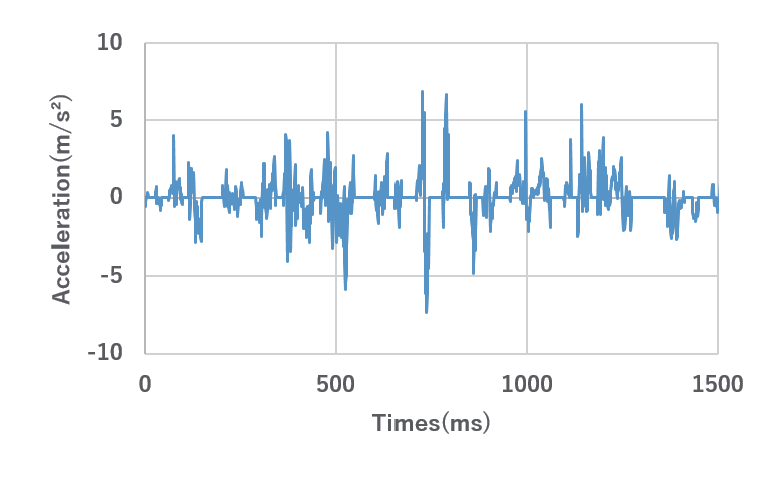
\includegraphics[width=12cm]{acc3.eps}
  \caption{パラメータ$e_x1(x)$を重畳した後の自作タイルテクスチャの振動情報}
  \label{acc3}
\end{center}
\end{figure}



% Local Variables:
% TeX-master: "main"
% mode: yatex
% End:
